\setchapterpreamble[u]{\vspace*{-3\baselineskip}\margintoc}
\chapter{Multifractal formalism for velocity fluctuations and singularities}
\labch{3}

\section{General Framework}
\subsection{Concept presentation}
Fractal structures appear in many physical phenomena such as turbulence, random walks and chaotic systems [Mandelbrot, 1982 ; Heitgen \& Saupe, 1988]. The concept of dimension plays a central role in their characterization. 

The usual dimension of an object is defined as the number of independent directions for a point moving in it. In this case, it is called the topological dimension $d_T$ and is a positive integer number. It is generally equal to\sidenote{sometimes smaller than} the dimension $d$ of the space in which the object is embedded. 

However, a smooth line and a random walk trajectory have the same topological dimension $d_T=1$, but very different characteristics since the latter densely fills a two-dimensional space. For this reason, it is necessary to introduce the \emph{fractal dimension} $\mathcal{D}_F$ of a geometrical object, considering the scaling of the number $\mathcal{N}(\epsilon)$ of hypercubes of size $\epsilon$ necessary to cover the object 
\begin{equation}
    \mathcal{N}(\epsilon)\simeq\epsilon^{-\mathcal{D}_F}\quad\epsilon\rightarrow0
\end{equation}
A more precise definition would require sophisticated methods, and lead to the introduction of the Hausdorff dimension, which can in some cases be different from $\mathcal{D}_F$. 

For a a smooth geometrical object\sidenote{e.g. a line, a sphere..} one has equality between topological and fractal dimensions, but scaling laws in nature should not be characterized by a mere single geometrical parameter. One has to consider the scaling properties of an appropriate density $\mu(\mathbf{x})$\sidenote{in many cases, a probability density} over the object. The coarse-grained measure can then be defined as [Mandelbrot, 1982]
\begin{equation}
    p_\epsilon(\mathbf{x})=\int_{B(\mathbf{x},\epsilon)}\mu(\mathbf{y}d\mathbf{y}
\end{equation}
Where $B(\mathbf{x},\epsilon)$ is a hypercube of linear size $\epsilon$ centered in the point $\mathbf{x}$ of the object. In general, we have the following scaling depending on the point $\mathbf{x}$, 
\begin{equation}
    p_\epsilon(\mathbf{x})\simeq\epsilon^\alpha,
\end{equation}
where $\alpha$ can differ from $\mathcal{D}_F$. In case of equality, the object is a perfect fractal. Otherwise, it can be regarded as a superposition of different fractal sets :
\begin{equation}
    \mathcal{F}(\alpha)=\{\mathbf{x}~such~that~p_\epsilon(\mathbf{x})\simeq\epsilon^\alpha~for~\epsilon\rightarrow0\}
\end{equation}
each one characterized by a different exponent $\alpha$. This object is then called multifractal [Parisi \& Frisch 1985, Benzi et al 1984, Paladin \& Vulpiani 1987a]. The fluctuations of the exponent $\alpha$ are ruled by a "probability" distribution which can be studied by analysing the scaling law of the moments
\begin{equation}
    \langle p_\epsilon^q\rangle\equiv\sum_{k=1}^{\mathcal{N}(\epsilon)}\bigg\{p_\epsilon(\mathbf{x}(k))\bigg\}^{q+1}\simeq\epsilon^{qd_{q+1}},
\end{equation}
where $\mathbf{x}(k)$ is centered in the $k$-th hypercube and the average $\langle\rangle$ is a weighted sum over the hypercubes\sidenote{$\displaystyle \langle(\dots)\rangle\equiv\sum(\dots)p_\epsilon(\mathbf{x}(k))$}. 
The $d_q$ are called generalized dimensions, and it can be shown [Grassberger 1985, Hentschel \& Procaccia 1993] that $\mathcal{D}_F=d_0$. In a homogeneous fractal, $d_q=\mathcal{D}_F\;  ;\;\forall q$, and standards arguments of probability theory [Grassberger 1983] ensure than $d_q$ is a non-increasing function of $q$. The exponent $d_1<d_0$ is the fractal dimension of the probability measure, of \emph{information dimension}. The number of hypercubes of size $\epsilon$ necessary to cover a subset $\mathcal{F}(\alpha)$ of the structure should behave in the scaling hypothesis as
\begin{equation}
    n(\alpha)\simeq\epsilon^{-f(\alpha)}
\end{equation}
Where $f(\alpha)$ becomes the fractal dimension of the subset $\mathcal{F}(\alpha)$ [Halsey et al 1996]. 
Since the probability measure of a hypercube with center $\mathbf{x}$ scales as equation (3), the weight $\mathcal{P}$ of the corresponding subset should scale as
\begin{equation}
    \mathcal{P}_\epsilon(\alpha)\simeq\epsilon^{H(\alpha)}\quad;\quad H(\alpha)=\alpha-f(\alpha)
\end{equation}
The function $H$ is an entropy function, as defined by the finite-time fluctuations of the Lyapunov exponent [Bohr \& Rand 1991]. The sum over the hypercubes can be estimated as
\begin{equation}
    \sum_{k=1}^{\mathcal{N}(\epsilon)}\bigg\{p_\epsilon(\mathbf{x}(k))\bigg\}^{q+1}\simeq\int d\alpha n(\alpha)\epsilon^{\alpha(q+1)}
\end{equation}


The saddle point method\sidenote{This method was largely developped by Debye, in Math. Ann., 67 (1909) and was later re-developed by many asymoptic analysis mathematicians, including Riemann. 
It consists on a "simple" method of computing the asymptotic expansion of integrals of the form 
\begin{equation}
    F(\lambda)=\int_\Gamma f(z)e^{\lambda S(z)}d z\tag{$\star$}\label{star}
\end{equation}
Where $\lambda>0,\lambda\rightarrow\infty$ is a large parameter, $\Gamma$ is a contour in the z-complex plane, and the functions $f(z),S(z)$ are holomorphic in a domain $D$ containing $\Gamma$. The zeroes of $S'(z)$ are called saddle points for $S(z)$. The method is as follows :
The contour $\Gamma$ is deformed to $\Tilde{\Gamma}$ with the same end-points and lying in $D$ such that $\max_{z\in\Tilde{\Gamma}}\Re{S(z)}$ is attained only at the saddle points or at the end of $\Tilde{\Gamma}$, also called the contour of steepest descent. 
The asymptotics of the integral (\ref{star}) along the path of steepest descent are calculated by means of the Laplace method and are equal to the sum of the contributions from the saddle points. The contribution $V_{z_0}(\lambda)$ from the $z_0$ point is an integral of the form of (\ref{star}) taken over a small arc of $\Tilde{\Gamma}$ containing the point $z_0$. If it is an interior point of $\Tilde{\Gamma}$ and $z_0$ is a saddle point with $S''(0)\neq0$, then 
\begin{equation}
    V_{z_0}(\lambda)=\sqrt{-\frac{2\pi}{\lambda S''(z_0)}}e^{\lambda S(z_0)}\big\{f(z_0)+\mathcal{O}(\lambda^{-1}\big\}
\end{equation}
The contour of steepest descent has the following property on it $\min_{\Gamma'}\max_{z\in\Gamma'}\Re{S(z)}$ is attained. 
Where the minimum is taken over all contours $\Gamma'$ lying in $D$ having the same end-points as $\Gamma$.} gives the domination of the integral value in the limit $\epsilon\rightarrow0$
\begin{equation}
    \langle p_\epsilon^q\rangle\simeq \epsilon^{\tilde{\alpha}q+H(\tilde{\alpha})},
\end{equation}
where $\tilde{\alpha}$ is given by the minimum condition
\begin{equation}
    \frac{d H(\alpha)}{d\alpha}\bigg|_{\alpha=\tilde{\alpha}}=q.
\end{equation}
The generalized dimensions are thus related to the $f(\alpha)$ function by the Legendre transformation 
\begin{equation}
    (q-1)d_q=\min_\alpha\big\{\alpha q-f(\alpha)\big\}
\end{equation}
Each order $q$ selects a particular exponent $\alpha$. The less probable $\alpha$ has the largest corresponding entropy function $H(\alpha)$. In particular, the entropy minimum is reached for $\alpha=d_1$, while the maximum of the $f(\alpha)$ curve is given by $d_0=\mathcal{D}_F$. 

\subsection{Practical definition}
Multifractal analysis aims at enhancing and enriching the characterization of a non-deterministic (ie, natural) fractal. The fractal dimension expresses the degree of \emph{complexity} of a given self-similar object, or structure, in particular in its ability to fill the hosting space. Being a non-integer number allows it to exceed the Euclidian dimension of the set (a fractal line, or filament is of fractal dimension higher than one ; similarly to sheets and bubbles, clouds), thus making it a meaningful indicator for quantifying the structure of complex, nested, convoluted structures which depart from the smoothness appearance of Euclidian shapes. The need of going beyong the simple and single descriptor leads to the formulation in the previous section of \emph{multifractal geometry}.

The definition of a set of orders $q\in\mathbb{R}$ [Hentschel \& Procaccia, 1983] was introduced to improve the characterization of chaotic attractors in dynamical systems. Sets which are not perfectly self-similar are those found in nature, as opposed to the well known Cantor set, or the Koch curve. Among various formulations of the generalized fractal dimensions, the box-counting approach is the most meaningful in the context of astrophysics, and image analysis. 

Let us start considering a set constituted by points\sidenote{e.g. black pixels in an image with a white background}, named \emph{measure} and cover it with boxes of size $\epsilon$. The probability of points contained in the $i$-th box is simplfy defined as the ratio of the corresponding number of points $\displaystyle P_i=N_i/N$. The $q$-th generalized dimension can then be defined as 
\begin{equation}
    d_q=\lim_{\epsilon\rightarrow0}\frac{1}{q-1}\frac{\log Z_q(\epsilon}{\log\epsilon}\quad;\quad Z_q(\epsilon)=\sum_iP_i^q
\end{equation}
The case $q=0$ recovers the classic expression of the box-counting monofractal dimension [Falconer, 2003].
The lower and upper limiting dimensions, $d_{(-\infty)}$ and $d_{(\infty)}$ are related to the regions of the set  which the measure is respectively \emph{most diluted}, and \emph{most concentrated}. 

The partition of function of the set has the scaling 
\begin{equation}
    Z_q(\epsilon)\propto\epsilon^{\tau_q},
\end{equation}
where $\tau_q$ is the \emph{correlation exponent of order} $q$ [Arrneodo, Bacry \& Muzy 1995]. Its relationship with $q$ can be written as
\begin{equation}
    \tau_q=qh(q)-E
\end{equation}
where $E$ is the Euclidian dimension of the volume hosting the fractal, the \emph{support of the measure} [Gu \& Zhou 2006]. For a monofractal, the \emph{Hurst exponent} $h(q)$ is constant, so that the relation between $ \tau_q$ and $q$ is linear. It is a function of $q$ in the multifractal case. 
Combining above equations leads to
\begin{equation}
    \tau_q=(q-1)d_q
\end{equation}
All the above definitions and considerations are strictly valid for a measure composed by discrete points, when a coverage of the support of the measure is performed. In the application to astronomical maps and observations, the measure is a 3D surface having values different from 0 at any point of its support which is a $m\times n$ pixels raster.

In this particular case, the probability $P_i$ becomes a sum of brightness of pixels falling in the $i$-th box, normalized by an integral over the entire map. This means that the astronomical view of the $0$-th order equation will always correspond to the Euclidian dimension $2$ of the support of the measure, rather than the true fractal dimension of the image. [Elia et al 2018]  

\subsection{Multifractal spectrum and practical derivation}
\emph{Multifractal spectrum} (MFS) is the name given by [Halsey 1986] to the \emph{singularity spectrum}. Considering a measure (astronomical, simulation-wise, or theoretical) emebdded in a support and covered with $\epsilon$-sized boxes. It the measure is adequatly multifractal, the probability $P_i$ scales with $\epsilon$ as a power law with exponent $\alpha_i$, the \emph{singularity strength}\sidenote{or, mathematically, the Holder exponent}. 

Given the fractal dimension $f(\alpha)$ of the subset of boxes having the singularity strength in the ($\alpha$,$\alpha+\delta\alpha$), the MFS is the curve of $f(\alpha)$ versus $\alpha$. It represents the contributions to the geometry provided by interwoven sets with different singularity strengths. 

Its relation with the generalized dimensions can be expressed via the Legendre transform (12) :\sidenote{From this relation, it is easy to derive certain properties of the $f(\alpha)$ curve : 
$$\frac{df}{d\alpha}=q\quad,\quad\frac{d^2f}{d\alpha^2}<0$$. The MFS is concave for any measure, and has infinite slopes for $q=\pm\infty$} 
\begin{equation}
    \alpha(q)=\frac{d}{dq}\tau_q \quad;\quad f(\alpha(q))=q\alpha(q)-\tau_q
\end{equation}
and can thus be calculated after derivation of all $(q,d_q)$ pairs. 

The MFS gives information about the relative importance of various fractal exponents present in the map, and its width indicates the range in which such exponents lie. The part corresponding to values $q>0$ (ie rising slope) characterizes overdense regions, because it magnifies the effect of large numbers, while $q<0$ represents the behaviour of low-density subsets. This generally result in an asymmetric shape of the MFS with respect to the peak position. [Puckovs \& Matvejevs 2012, Belete et al 2019]

The first choice in the analysis comes from the depth of $q$-orders. The probed ranged can freely be asymmetric, in varing steps, chosen as to minimize the calculation errors, and better sample critical regions for multifractal descriptors. 

The plot of $\tau_q$ vs $q$ does not present linear behaviour, but a typically multifractal behaviour with two different slopes for the two $q>0$ and $q<0$ regimes. The transition zone should explicit a non-linear behaviour [Movahed et al 2011, Xie et al 2015]. Similarly, the $d_q$ vs $q$ curve is far from being constant [Meneveau \& Sreenivasan 1987] confirming that the analysed image presents a multifractal character\sidenote{rather than a monofractal one}. 

Once these two parameters are computed, a method developed by [Chhabra \& Jensen 1999] and first applied by [Chappell \& Scalo 2001] to astrophysics context revolves as follows. The coarse-grained moments of the image can be defined by
\begin{equation}
    \mu_i(q,\epsilon)=\frac{P_i^q(\epsilon)}{\sum_iP_i^q(\epsilon)}
\end{equation}
Thus defining $\alpha$ and $f(\alpha)$ with respect to $q$ via
\begin{equation}
    \begin{cases}
\displaystyle    \alpha(q)=\lim_{\epsilon\rightarrow0}\frac{1}{\log\epsilon}\sum_i\mu_i(q,\epsilon)\log P_i^q(\epsilon)\\
    \displaystyle f(q)=\lim_{\epsilon\rightarrow0}\frac{1}{\log\epsilon}\sum_i\mu_i(q,\epsilon)\log \mu_i(q,\epsilon)\\
    \end{cases}
\end{equation}
In practice, the quantites whose limit is calculated in the RHS show linear behaviour [Elia 2018, Belete 2019], meaning that the uncertainties associated with the values of $\alpha(q)$ and $f(\alpha(q))$ mainly depend on the quality of the linear fit. Even though the MFS was initially introduced as stated in equations (6) to (12), we will refer to the [Chhabra \& Jensen 1999] computing method. 

\subsection{Properties of the multifractal spectra}
The two most important\sidenote{and immediate} information items from this spectra are the width $\Delta\alpha=\alpha_{max}-\alpha_{min}$ and the symmetry in the shape of $\alpha$ defined as $A=(\alpha_{max}-\alpha_0)/(\alpha_0-\alpha_{min})$, where $\alpha_0$ is the value of $\alpha$ when $f(\alpha)$ assumes its maximum value. The width of such a spectrum is the measure of the degree of multifractality [Ashkenazy 2003, Shimizu 2002]. Smaller values of $\Delta\alpha$ indicate the monofractal limit, while larger values indicate the strength of multifractal behaviour in the signal [Telesca 2004].


For the symmetry in the shape of $\alpha$, there are only three possible configurations. 
Either it is right-truncated ($A>1$) or left-truncated ($A<1$), or perfectly symmetric\sidenote{This case is highly unlikely in any physical system} ($A=1$). A perfectly symmetric spectrum originates [Ihlen 2012] from the leveling of the $q$-th order generalized Hurst exponent for both positive and negative $q$ values. This leveling would mean that the $q$-th order fluctuation is \emph{insensitive} to the magnitude of the local fluctuation. 

Conversely, when the multifractal structure is sensitive to small scale fluctuations, with large magnitudes, the spectrum will be found with a right-truncation ; the left-side truncation is favored when the multifractal structure is sensitive to local fluctuations with small magnitudes. 

The width and shape of the MFS are able to classify small and large (intermittency) fluctuations and determine the degree of multifractality signature in a given structure\sidenote{or signal}. 

\begin{figure}
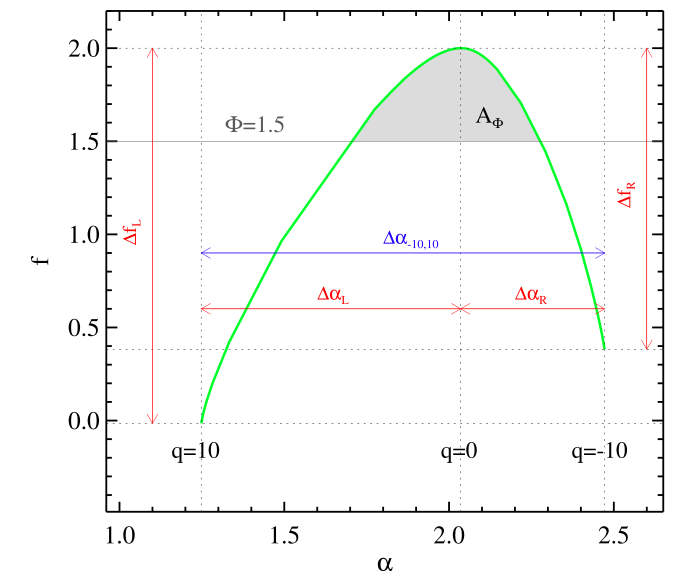
\includegraphics[width=.85\linewidth]{3/setsumei.png}
\caption{Faire un long caption expliquant tous les paramètres...}
\end{figure}
From the multifractal spectrum, many parameters and informations can be derived :
\begin{itemize}
\item{Qualitative analysis}
\item{Dimensional diversity, maximum singularity strength}
\item{Peak position}
\item{MFS width}
\item{Tails asymetry}
\item{Horizontal|Vertical Balance}
\item{Generalized fractal dimensions' approach}
\end{itemize}

\section{Analysis code}
\subsection{Presentation}
\subsection{Low-complexity verifications}
\subsection{Complete structures}

\section{Spectra in the inertial region}

\subsection{Log-normal (KO) exponent spectrum}
In general, the longitudinal velocity signal presents scale-invariant properties, and it is thus expected (previous chapter) that structure functions do behave according to power laws :
\begin{equation}
    \langle(\delta_\ell u)^q\rangle\simeq\ell^{\zeta_q^E}
\end{equation}
A log-normal model for non-trivial dissipation fluctuations results in a non-linear quadratic model for the exponent spectrum $\zeta_q^E$, which can be defined with the linear coefficient $c_1$ and the intermittence (non-linearity) coefficient $c_2$ :
\begin{equation}
    \zeta_q^E=c_1q-c_2\frac{q^2}{2}
\end{equation}
The linear term should be very close to the Kolmogorov K41 predictions ($c_1=1/3$), and both coefficients are constrained under the condition 
\begin{equation}
    \zeta_3^E=1
\end{equation}
Which comes directly from the Navier-Stokes' equation, as the \emph{four-fifth law} :
\begin{equation}
    \lim_{\ell\rightarrow0}\lim_{\nu\rightarrow0}\frac{\langle(\delta_\ell u)^3\rangle}{\ell}=-\frac{4}{5}\langle\epsilon\rangle
\end{equation}
One can thus derive the relation
\begin{equation}
    c_1=\frac{1}{3}+\frac{3}{2}c_2,
\end{equation}
to which nearly every experimental, numerical and observational shows good compatibility. 
Slightly redefining the previously introduced refined-similarity hypothesis 
\begin{equation}
    (\delta_\ell u)^q\simeq\ell^{q/3}\epsilon_\ell^{q/3},
\end{equation}
which now accounts for the fluctuations of the dissipation averaged over a $\ell$-size tpological ball. This means, for a $\vec{r}$ point in space,
\begin{equation}
    \epsilon_\ell(\vec{r})=\frac{3}{4\pi\ell^3}\int_{|\vec{r'}-\vec{r}|<\ell}\epsilon(\vec{r'})d^3r'
\end{equation}
is a quantity that should depend upon the center of the $\ell$-ball. The KO62 scale-invariance implies the scaling via the exponent spectrum 
\begin{equation}
    \langle(\epsilon_\ell)^q\rangle\simeq\ell^{\tau_q^E}
\end{equation}
Therefore, the anormal\sidenote{intermittent} behaviour of velocity fluctuations across scales, knowning the dissipation fluctuations spectrum, is given by\sidenote{In K41, the fluctuations of $\epsilon_\ell$ are independent of the scale $\ell$, and thus $\tau_q=0$. This is in agreement with the expected linear spectrum $\zeta_q=q/3$.}
\begin{equation}
    \zeta_q^E=\frac{q}{3}+\tau_{q/3}^E
\end{equation}
A log-normal statistics\sidenote{According to Obhukov77, this choice is not specifically restrictive, since the random variable $\epsilon_\ell$ only takes strictly positive values. Mathematical probability theorems guarantee that any stricty positive random variable can be approximated, at least for its few first moments, by a log-normal variable} for $\epsilon_\ell$, for all intertial scales $\ell\in\lbrack\eta_K,L\rbrack$ assumes the form
\begin{equation}
    \mathcal{P}_{\epsilon_\ell}(\epsilon_\ell)d\epsilon_\ell=\mathcal{P}_{\ln\epsilon_\ell}(\ln\epsilon_\ell)d\ln\epsilon_\ell=\sqrt{\frac{1}{2\pi\sigma_\ell^2}}\exp\bigg[\frac{(\ln\epsilon_\ell-m_\ell)^2}{2\sigma_\ell^2}\bigg]d\ln\epsilon_\ell
\end{equation}

Its moments are an immediate consequence of the probability distribution :
\begin{equation}
   \langle(\epsilon_\ell)^q\rangle =\int_\mathbb{R}(\epsilon_\ell)^q\mathcal{P}_{\ln\epsilon_\ell}(\ln\epsilon_\ell)d\ln\epsilon_\ell=\exp\bigg[\frac{1}{2}q(q\sigma_\ell^2+2m_\ell)\bigg]
\end{equation}

Since the local dissipation, and the averaged dissipation over a $\ell$-ball are identical in mean, 
\begin{equation}
    m\ell=\ln\langle\epsilon\rangle-\frac{\sigma_\ell^2}{2}
\end{equation}
Thus, the only remaining parameter is the variance of $\ln\epsilon_\ell$, 
\begin{equation}
\langle(\epsilon_\ell)^q\rangle=\langle\epsilon\rangle^q\exp\bigg[\frac{1}{2}q(q-1)\sigma_\ell^2\bigg]    
\end{equation}
The variance should be chosen proportional to the scale, ie
\begin{equation}
\sigma_\ell^2=9c_2\ln\frac{L}{\ell}    
\end{equation}
in which the $L$ characteristic scale, integral scale, constrains the limit of validity of the relation (being the upper limit)\sidenote{This means for scales $\ell\geq L$, we have $\sigma_\ell^2=0$.}. 

The dissipation moments to obey
\begin{equation}
    \langle(\epsilon_\ell)^q\rangle=\langle\epsilon\rangle^q\left(\frac{\ell}{L}\right)^{\tau_q^E}\quad with\quad \tau_q^E=\frac{9}{2}c_2q(1-q)
\end{equation}
The refined similarity hypothesis gives the exponent spectrum for the velocity structure functions as
\begin{equation}
    \zeta_q^E=\left(\frac{1}{3}+\frac{3}{2}c_2\right)q-c_2\frac{q^2}{2}
\end{equation}

\subsection{Defining the "physical" Singularity spectrum}

The general framework for singularity analysis of a distribution, notably by wavelet transform, and the generalisation of multifractal formalism for distributions and measures was developped by Parisi and Frisch 85-88-91. The phenomenon of turbulent intermittence can also be described by this singularity formalism, which applies naturally to the spatial velocity profile $u(x)$ :
\begin{equation}
    \delta_\ell u(x)=u(x+\ell)-u(x)\simeq\ell^{h(x)}\quad when\;\ell\rightarrow0,
\end{equation}
where $h(x)$ is the Hölder unique exponent\sidenote{$h=1/3$ in the monofractal K41 theory}.
The \emph{spectrum of singularities} $\mathcal{D}^E(h)$ is defined as :
\begin{equation}
    \mathcal{D}^E(h)=d_F(\{x_0\in\mathbb{R}\,|\,h(x_0)=h\}
\end{equation}
where $d_F$ represents the fractal dimension\sidenote{ie, the Haussdorf dimension of the space in question}. In the K41 theory, the velocity signaul is singular in each point with the same Hölder exponent $1/3$, which means that for every $x$, the velocity increment over a distance $\ell$, namely $\delta_\ell u(x)$ behaves like $\ell^{1/3}$.
Therefore, the ensemble $\{x\in\mathbb{R}\,|\,h(x)=h\}$ is exactly $\mathbb{R}$ for $h=1/3$ and the spectrum $\mathcal{D}^E(h)$ contains trhe only point $\mathcal{D}^E(h=1/3)=1$.\sidenote{by convention, $\mathcal{D}(h)^E=-\infty$ for $h\neq1/3$}

The multifractal formalism associates a probability law, and behaviour to the $h$ exponent. Therefore, given a scale $\ell$, the probability $\mathbb{P}_\ell^i(h)$ that the velocity increment at this scale behaves as $\simeq\ell^h$ is directly linked with the fractal dimension of the ensemble of points for which this singularity exists :
\begin{equation}
    \mathbb{P}_\ell(h)\simeq\ell^{1-\mathcal{D^E(h)}}
\end{equation}

Therefore, the intermittency property of velocity fluctuations can be written as the existence of many singularity exponents (or forces) attached with a certain probability. In fact, every turbulent spectrum studied presents a \emph{continuum} of these exponents. This formalism is based on a local interpretations of scale-invariant properties or the field, via the (localà Hölder exponent, fluctuationg from one point to another. 

The link between the global power-law behaviour of structure functions, and then singular local behaviour of the velocity profile is held by the Legendre transform\sidenote{This relation is demonstrated as follows. Taking the structure functions in the limit $\ell\rightarrow0^+$ and applying the neck method \begin{align*}
    \langle(\delta_\ell u)^q\rangle&\simeq\ell^{\zeta_q^E}\\
                                   &\simeq\int\ell^{qh}\times\ell^{1-\mathcal{D}^E(h)}dh\\
                                   &\simeq\ell^{\min_h\big[qh+1-\mathcal{D}^E(h)\big]}
\end{align*}}
\begin{equation}
    \zeta_q^E=\min_h\big[qh+1-\mathcal{D}^E(h)\big]
\end{equation}

Since we are working with physical functions, continually derivable, the transform can be rewritten as
\begin{equation}
    \begin{cases}
    \displaystyle q=&d\mathcal{D}^E(h)/dh\\
    \displaystyle \zeta_q^E=&hq+1-\mathcal{D}^E(h)
    \end{cases}
\end{equation}

The physical multifractal formalism consists in the inverse transform of the exponent spectrum
\begin{equation}
    \mathcal{D}^E(h)=\min_h\big[1+qh-\zeta_q^E\big]
\end{equation}
which can also be rewritten
\begin{equation}
    \begin{cases}
    \displaystyle h=&d\zeta_q^E(h)/dq\\
    \displaystyle \mathcal{D}^E(h)=&1+hq-\zeta_q^E(h)
    \end{cases}
\end{equation}

The above relation immediately gives the singularity spectrum for KO62 :
\begin{equation}
    \mathcal{D}^E(h)=1-\frac{(h-c_1)^2}{2c_2}
\end{equation}

The following calculations are based on a number of definitions taken from the previous sections. Its main application condition is the ergodic hypothesis, largely developped by Tennekes and Lumley. More details on this hypothesis and its consequences on the characteristic function representing the turbulent velocity, and that representing local dissipation fields, can be found in Appendix B. 

\section{Singularity spectrum in Eulerian and Lagrangian dissipation}
Taking into account non-trivial fluctuations of the mean dissipation $\epsilon_\ell$, as stated in equations....., the KO62 log-normal cascade model was developped, mainly in order to explain the intermittent nature of velocity fluctuations in different scales.
The constraining power-laws on $\epsilon_\ell$ in the inertial regime can be extended to dissipation scales thanks to the previously introduced multifractal formalism. In the following, the exponent$^E$ merely refers to Eulerian considerations.

\subsection{Exposant spectrum $\tau_q^E$ and singularity spectrum $f^E(\alpha)$}
In the interial regime, the mean dissipation's fluctuations exhibit scale-invariant properties that could be described by
\begin{equation}
    \langle\epsilon_\ell^q\rangle=\langle\epsilon\rangle^q\left(\frac{\ell}{L}\right)^{\tau_q^E}
\end{equation}
Where, refering to the $\mu^E$ intermittency coefficient of the log-normal approach\sidenote{In fact, it is only linked to the intermittency coefficient of the Eulerian longitudinal velocity $c_2^E$, thanks to the aforementionned refined-similarity hypothesis $$\mu^E=9c_2^E\simeq0.225$$}
\begin{equation}
    \tau_q^E=\frac{1}{2}\mu^Eq(1-q)
\end{equation}
The multifractal formalism thus gives a local interpretation of this behaviour in terms of power-law, i.e.
\begin{equation}
    \epsilon_\ell=\langle\epsilon\rangle\left(\frac{\ell}{L}\right)^{\alpha-1}
\end{equation}
Where $\alpha$ is an exponent that should depend on spatial position and characterizes the singularity strength of the measure $\epsilon_\ell$. Calling $\mathbb{P}_\ell^i(\alpha)$ the probability density function of $\alpha$ in the intertial reggime, it is then easily linked with the singularity spectrum $f^E(\alpha)\propto\left(\frac{\ell}{L}\right)^{1-f^E(\alpha)}$
The main result of the multifractal formalism revolve around the equivalency between the singularity spectrum and the exponent spectrum, via Legendre transform : 

\begin{equation}
    \tau_q^E=\min_\alpha\bigg[q(\alpha-1)+1-f^E(\alpha)\bigg]\iff f^E(\alpha)=\min_q\bigg[q(\alpha-1)+1-\tau_q^E\bigg]
\end{equation}

This means that the log-normal spectrum gives a quadratic singularity spectrum 
\begin{equation}
    f^E(\alpha)=1-\frac{1}{2\mu^E}\left(\alpha-\left(1+\frac{\mu^E}{2}\right)^2\right)
\end{equation}
and has for support ($f^E(\alpha)\geq0$) the interval\sidenote{It is interesting to note that this interval is actually a single point $\alpha=1$ in the monofractal definition of K41 (in which $\mu^E=0$. The entire spectrum becomes a $\delta$-function.} $$ \alpha\in\bigg[1+\frac{\mu^E}{2}-\sqrt{2\mu^E}\;;\;1+\frac{\mu^E}{2}+\sqrt{2\mu^E}\bigg]$$

\subsection{Typical dissipative Eulerian scales}
Implementing dissipaton scales requires the use of the local Reynolds number $\mathcal{R}_\ell$. It is known that the dissipative scale $\eta(h)$ varies when the longitudinal velocity increments' fluctuations are intermittent, ie, when the $h$ exponent varies spatially.
In a similar fahion, then dissipative scale can be parametrized by the $\alpha$ exponent. This implies our main driving factor is $\epsilon_\ell$ rather than $\delta_\ell u$. The Reynolds number is defined with typical values in the integral scale $L$, ie a characteristic velocity of $\langle\epsilon\rangle^{1/3}L^{1/3}$, the $L$ scale, and viscosity $\nu$, thus
\begin{equation}
    \mathcal{R}_e=\frac{\langle\epsilon\rangle^{1/3}L^{4/3}}{\nu}
\end{equation}
The local Reynolds number can, using equations() be written
\begin{equation}
    \mathcal{R}_\ell=\frac{\epsilon\ell^{1/3}\ell^{4/3}}{\nu}=\left(\frac{\ell}{L}\right)^{\frac{3+\alpha}{\alpha}}\times\mathcal{R}_e,
\end{equation}
thus constraining the dissipative scale $\eta$ to fluctuate since the local Reynold number at this scale should be a constant $\mathcal{R}_\star$.
Thus\sidenote{Which is compatible with the monofractal K41 prediction $$\eta(\langle\alpha\rangle\simeq1)\propto L\mathcal{R}_e^{-3/4}$$}
\begin{equation}
\eta(\alpha)=L\left(\frac{\mathcal{R}_e}{\mathcal{R}_\star}\right)^{\frac{-3}{3+\alpha}}
\end{equation}

In the limit of infinitely small $\ell$ scales, the mean dissipation $\epsilon_\ell$ coincides with the local dissipation $\epsilon$. Therefore, the statistics of $\epsilon_\ell$ saturates in the dissipation region. This intrinsic limit in scaling is naturally taken into account by the multifractal formalism, respecing the continuity of $\epsilon_\ell$ in $\ell=\eta(\alpha)$.
Thu, the multifractal formalism give the prediction

\begin{equation}
    \epsilon(\alpha,\mathcal{R}_e)=\langle\epsilon\rangle\left(\frac{\eta(\alpha)}{L}\right)^{\alpha-1}
\end{equation}
where the exponent $\alpha$'s probability density function is given by
\begin{equation}
    \mathbb{P}_\ell^d(\alpha,\mathcal{R}_e,f^E(\alpha))\propto\left(\frac{\eta(\alpha)}{L}\right)^{1-f^E(\alpha)}
\end{equation}

Despite the Eulerian approach being generally considered in simulations and theoretical works, the fluctuations of the dissipation $\epsilon_\tau$, as seen by a fluid particle alongside its trajectory during a time $\tau$ might hold significant information as well.
\subsection{Exposant spectrum $\tau_q^L$ and singularity spectrum $f^L(\alpha)$}
Similarly to the Eulerian case, the scale fluctuations of the mean dissipation exhibit, in the intertial regime, scale-invariant properties : 
\begin{equation}
    \langle\epsilon_\tau^q\rangle=\langle\epsilon\rangle\left(\frac{\tau}{T}\right)^{\tau_q^L}
\end{equation}
The $\mu^L$ coefficient, defined in the quadratic form 
\begin{equation}
    \tau_q^L=\frac{1}{2}\mu^Lq(1-q)
\end{equation}
is this time linked to the $c_2^L$ coefficient of the Lagrangian speed, ie $\mu^L=4c_2^L\simeq0.32$ in the log-normal model. 
The power-law behaviour for the moments of the mean dissipation are given by a similar exponent than in the previous section
\begin{equation}
    \langle\epsilon_\tau=\langle\epsilon\rangle\left(\frac{\tau}{T}\right)^{\kappa-1}
\end{equation}
which fluctuates \emph{temporaly}\sidenote{as opposed to spatially in the previous section}, and of which the probability density in the intertial regime is given in terms of the singularity spectrum by
\begin{equation}
    \mathbb{P}^i_\tau(\kappa)\propto\left(\frac{\tau}{T}\right)^{1-f^L(\kappa)}
\end{equation}
These two spectrum are once again Legendre Transforms of one another, and the singularity spectrum exhibit similar quadratic behaviour\sidenote{$$f^L(\kappa)=1-\frac{1}{2\mu^L}\left(\kappa-\left(1+\frac{\mu^L}{2}\right)^2\right)$$}, although the intermittency coefficient becomes the Lagrangian one. 

\subsection{Typical dissipative Lagrangian scales}

Using time-scaling quantites, the Reynolds number takes the form
\begin{equation}
    \mathcal{R}_e=\frac{\langle\epsilon\rangle T^2}{\nu}
\end{equation}
The local Reynold number is, this time,
\begin{equation}
    \mathcal{R}_\tau=\frac{\epsilon_\tau\tau^2}{\nu}=\left(\frac{\tau}{T}\right)^{\kappa+1}\mathcal{R}_e
\end{equation}
The dissipative scale thus fluctuates as
\begin{equation}
    \tau_\eta(\kappa)=T\left(\frac{\mathcal{R}_e}{\mathcal{R}_\star'}\right)^{\frac{-1}{1+\kappa}}
\end{equation}

Finally, the formalism's prediction in Lagrangian description is
\begin{equation}
    \epsilon(\kappa,\mathcal{R}_e)=\langle\epsilon\rangle\left(\frac{\tau_\eta{\kappa}}{T}\right)^{\kappa-1}
\end{equation}

\section{Statistical links between both descriptors}
\subsection{Spectrum unification}
The ergodic hypothesis of Tennekes-Lumley implies that the caracteristic functions of both descriptors are to be identical.
Thus, the $q$-order moments of these two quantites should also be so :
\begin{equation}
    \langle\epsilon(\vec{x},t)^q\rangle=\langle\epsilon(\vec{r_0},t)^q\rangle
\end{equation}
Using previous developments, the $q$-order moment of both quantities can be calculated :\\

\begin{fullwidth}\begin{equation}
    \displaystyle \langle\epsilon(\vec{x},t)^q\rangle\propto\langle\epsilon\rangle^q\int_{\alpha_{min}}^{\alpha_{max}}\left(\frac{\mathcal{R}_e}{\mathcal{R}_\star}\right)^{\frac{-3}{3+\alpha}\left(q(\alpha-1)+1-f^E(\alpha)\right)}d\alpha\propto\left(\frac{\mathcal{R}_e}{\mathcal{R}_\star}\right)^{\min_\alpha\bigg[\frac{-3}{3+\alpha}\left(q(\alpha-1)+1-f^E(\alpha)\right)\bigg]}
\end{equation}\end{fullwidth}

\begin{fullwidth}\begin{equation}
    \displaystyle \langle\epsilon(\vec{r_0},t)^q\rangle\propto\langle\epsilon\rangle^q\int_{\kappa_{min}}^{\kappa_{max}}\left(\frac{\mathcal{R}_e}{\mathcal{R}_\star'}\right)^{\frac{-1}{1+\kappa}\left(q(\kappa-1)+1-f^L(\kappa)\right)}d\kappa\propto\left(\frac{\mathcal{R}_e}{\mathcal{R}_\star'}\right)^{\min_\kappa\bigg[\frac{-1}{1+\kappa}\left(q(\kappa-1)+1-f^L(\kappa)\right)\bigg]}
\end{equation}\end{fullwidth}

The minimisation problems' solutions can be denoted by $\alpha'(q),\kappa'(q)$, which verify
\begin{equation}
    \begin{cases}
    \displaystyle\min_\kappa\bigg[\frac{-3}{3+\alpha}\left(q(\alpha-1)+1-f^L(\alpha)\right)\bigg]=-3\frac{(q(\alpha'-1)+1-f^L(\alpha')}{3+\alpha'}&\\
    \displaystyle\min_\kappa\bigg[\frac{-1}{1+\kappa}\left(q(\kappa-1)+1-f^L(\kappa)\right)\bigg]=-\frac{(q(\kappa'-1)+1-f^L(\kappa')}{1+\kappa'}&\\
    \end{cases}
\end{equation}

Allowing the conditions 
\begin{equation}
    \forall q,\quad\frac{\kappa'(q)-1}{\kappa'(q)+1}=3\frac{\alpha'(q)-1}{\alpha'(q)+3}\;and\;\frac{1-f^L(\kappa'(q))}{\kappa'(q)+1}=3\frac{1-f^3(\alpha'(q))}{\alpha'(q)+3}
\end{equation}
Then we have the relation $\forall \kappa$,
\begin{equation}
    f^L(\kappa)=-\frac{1}{2}\kappa+\left(1+\frac{1}{2}\kappa\right)f^E\left(\frac{3\kappa}{2+\kappa}\right)
\end{equation}
Which can be reversed as 
\begin{equation}
    f^E(\alpha)=\frac{1}{3}\kappa+\left(1-\frac{1}{3}\alpha\right)f^L\left(\frac{2\alpha}{3-\alpha}\right)
\end{equation}

\subsection{Dimensional statistical arguments}
Many studies of experimental and numerical velocity signals do exhibit rather more intermittency in the Lagrangian case than in the Eulerian one, giving rather Reynolds-free and experiment-free coefficients $c_2^E=0.025\pm0.003$, and $c_2^L=0.08\pm0.01$. 
Since intermittency is a characteristic of the evolution of scales of statistics and observables (velocity, dissipation..), a relationship between the spatial and temporal scales for which the flow exhibits a similar complexity reconciles both models; 
That would imply that both local Reynolds number $\mathcal{R}_\ell=\mathcal{R}_\tau$.
This means,
\begin{equation}
    \ell^2\tau^{-3}=(\epsilon_\tau)^{3/2}(\epsilon_\ell)^{-1/2}
\end{equation}
In a monofractal K41 description of turbulence, the exponents $(\alpha,\kappa)=(1,1)$ are unique, and the local Reynolds number do not fluctuate. The dissipation scales are scale-dependent. In a similar complexity, the previous equation becomes
\begin{equation}
    \ell^2\tau^{-3}\simeq\langle\epsilon\rangle
\end{equation}
At these scales $\ell,\tau$, the mean dissipation are equal in law, as the flow should dissipate in a time $t$ the same energy quantity as that on a scale $\ell$ along a Lagrangian trajectory, that is, 
\begin{equation}
    \forall q,\;\langle\epsilon_\ell^q\rangle=\langle\epsilon_\tau^q\rangle
\end{equation}
This simple argument leads to
\begin{equation}
    \tau_q^L=\frac{3}{2}\tau_q^E
\end{equation}
Admitting the foremost equation in first approximation when the flow is intermittent allows for the generalization of the above equation to multifractal formalism. Thus, in the log-normal descriptor, using the equations of the previous chapter, the intermittence coefficient are linked by
\begin{equation}
    \mu^L=\left(\frac{3}{2}\right)\mu^E
\end{equation}
In the refined-similarity hypothesis, the velocity fluctuations can thus be generalized as
\begin{equation}
    \zeta_q^L=\frac{3}{2}\left(\zeta^E_{3q/2}-\frac{q}{2}\right)+\frac{q}{2}
\end{equation}
This would lead to the link $\displaystyle c_2^L=\left(\frac{3}{2}\right)^3c_2^E$, which, although a simple dimensional argument, rather agrees with experimental and numerical values\sidenote{$c_2^L/c_2^E=3.20\simeq(3/2)^3=3.37$}.   


\subsection{E-L Transform of velocity singularities}
In the previous section, we derived a relation between intermittency coefficients of the log-normal model for velocity fluctuations (i) referring to dimensional arguments (ii) neglecting intermittent corrections between characteristic spatial and temporal scales, (iii) using a phenomenological reltation, and (iv) invoking the refined-similarity hypothesis. 

In order to derive a relationship between the singularity spectra $\mathcal{D}^E(h)$ and $\mathcal{D}^L(h)$, using the ergodicity hypothesis of Tennekes-Lumey (appendix), and inserting intermittent corrections. 

The description of the mean dissipation $\epsilon_\ell$ and the longitudinal velocity increment $\delta_\ell u$ can be written
\begin{equation}
    h=\frac{\alpha}{3}\;;\;\mathcal{D}^E(h)=f^E(\alpha)+d-1\quad and\quad \zeta_q^E=\frac{q}{3}+\tau^E_{q/3}
\end{equation}
where $d$ is the Euclidian dimension of the space in which the velocity is roaming.
Similarly, in Lagrangian descriptors,
\begin{equation}
    h=\frac{\kappa}{2}\;;\;\mathcal{D}^L(h)=f^L(\kappa)+d-1\quad and\quad \zeta_q^L=\frac{q}{2}+\tau^L_{q/2}
\end{equation}

In a 1D (e.g. radial) velocity profile, we then have
\begin{equation}
    \mathcal{D}^L(h)=-h+(1+h)f^E\left(\frac{3h}{1+h}\right)
\end{equation}
Posing $\alpha=3h/(1+h)$, we have the relationship 
\begin{equation}
    \mathcal{D}^L(h)=-h+(1+h)\mathcal{D}^E\left(\frac{h}{1+h}\right)
\end{equation}
which can be inverted as 
\begin{equation}
    \mathcal{D}^E(h)=h+(1-h)\mathcal{D}^L\left(\frac{h}{1-h}\right)
\end{equation}

\section{Interpretation and validity region}
\subsection{Monofractal limit}
THe previous relationships clearly imply that there is equivalence in monofractality for both description of velocity fluctuation. Therefore, the above spectra is valid in the K41 model range, and reconciles both descriptors. 

\subsection{Log-normal Model}
In the KO62 description, the Eulerian singularity spectrum ought to assume the quadratic shape
\begin{equation}
    \mathcal{D}^E(h)=1-\frac{(h-c_1^E)^2}{2c_2^E}
\end{equation}
It is particularly in agreement with many observational and numerical data, using the parameters $c_2^E=0.025$ and $c_1^E=1/3+3c_2^E\simeq0.37$. 
The Lagrangian spectrum is given by the previously developped transformation, which is non-linear. 
Therefore the Lagrangian spectrum is not quadratic, and the log-normal model cannot be applied to both decriptors of the flow. To quantify their difference, we can derive the exponent spectrum $\zeta_q^L$, which is the Legendre transform of $\mathcal{D}^L(h)$ :
\begin{equation}
    \zeta_q^L=\min_h\big[qh+1-\mathcal{D}^L(h)\big]
\end{equation}
This minimum can be solved thanks to the series expansion 
\begin{fullwidth}\begin{equation}
    \zeta_q^L=\frac{c_1^E}{1-c_1^E}q-\frac{c_2^E}{(1-c_1^E)^3}\frac{q^2}{2}+3\times\frac{(c_2^E)^2}{(1-c_1^E)^5}\frac{q^3}{3!}-15\times\frac{(c_2^E)^3}{(1-c_1^E)^7}\frac{q^4}{4!}+o(q^4)
\end{equation}\end{fullwidth}
And we have the identities
\begin{equation}
    c_1^L=\frac{c_1^E}{1-c_1^E}\quad and\quad c_2^L=\frac{c_2^E}{(1-c_1^E)^3}
\end{equation}

\subsection{Log-poisson Model}
In this case, the Eulerian spectrum of singularities can be written
\begin{equation}
    \mathcal{D}^E(h)=-1+A\left(h-\frac{1}{9}\right)-B\left(h-\frac{1}{9}\right)\ln\left(h-\frac{1}{9}\right)
\end{equation}
Where we get
\begin{equation}
    A=3\times\left(\frac{1+\ln\ln(3/2)}{\ln(3/2)}-1\right)\quad and\quad B=\frac{3}{\ln(3/2)}
\end{equation}

The exponent spectrum can then be derived as
\begin{equation}
    \zeta_q^L=\frac{q}{9}+2\times\left(1-\left(\frac{2}{3}^{q/3}\right)\right)
\end{equation}

By comparison, the expansion becomes
\begin{equation}
    \zeta_q^E=\bigg[\frac{1}{9}-\frac{2}{3}\ln\left(\frac{2}{3}\right)\bigg]q-\sum_2^\infty\frac{2}{3^n}\bigg[\ln\left(\frac{2}{3}\right)\bigg]^n\frac{q^n}{n!}
\end{equation}
We thus have the following models :
\begin{equation}
    \begin{cases}
    Log-Normal&\displaystyle\zeta_q^E=0.370(\pm0.005)q-0.025(\pm0.003)\frac{q^2}{2}+o(q^3)\\
    Log-Poisson&\displaystyle\zeta_q^E=0.381q-0.0365\frac{q^2}{2}-0.005\frac{q^3}{3!}+o(q^4)\\
    \end{cases}
\end{equation}
Where the log-normal values are taken as the experimental ones for comparison purposes (thus not exceeding order 3).
In Lagrangian terms, we can write :
\begin{equation}
    \begin{cases}
    Log-Normal&\displaystyle\zeta_q^L=0.589q-0.100\frac{q^2}{2}+0.019\frac{q^3}{3!}-0.006\frac{q^4}{4!}+o(q^4)\\
    Log-Poisson&\displaystyle\zeta_q^L=0.617q-0.154\frac{q^2}{2}+0.078\frac{q^3}{3!}-0.061\frac{q^4}{4!}+o(q^4)\\
    \end{cases}
\end{equation}